\begin{figure}[b]
    \vskip -1.5\baselineskip
    \centering
    \begin{subfigure}[t]{0.32\textwidth}
        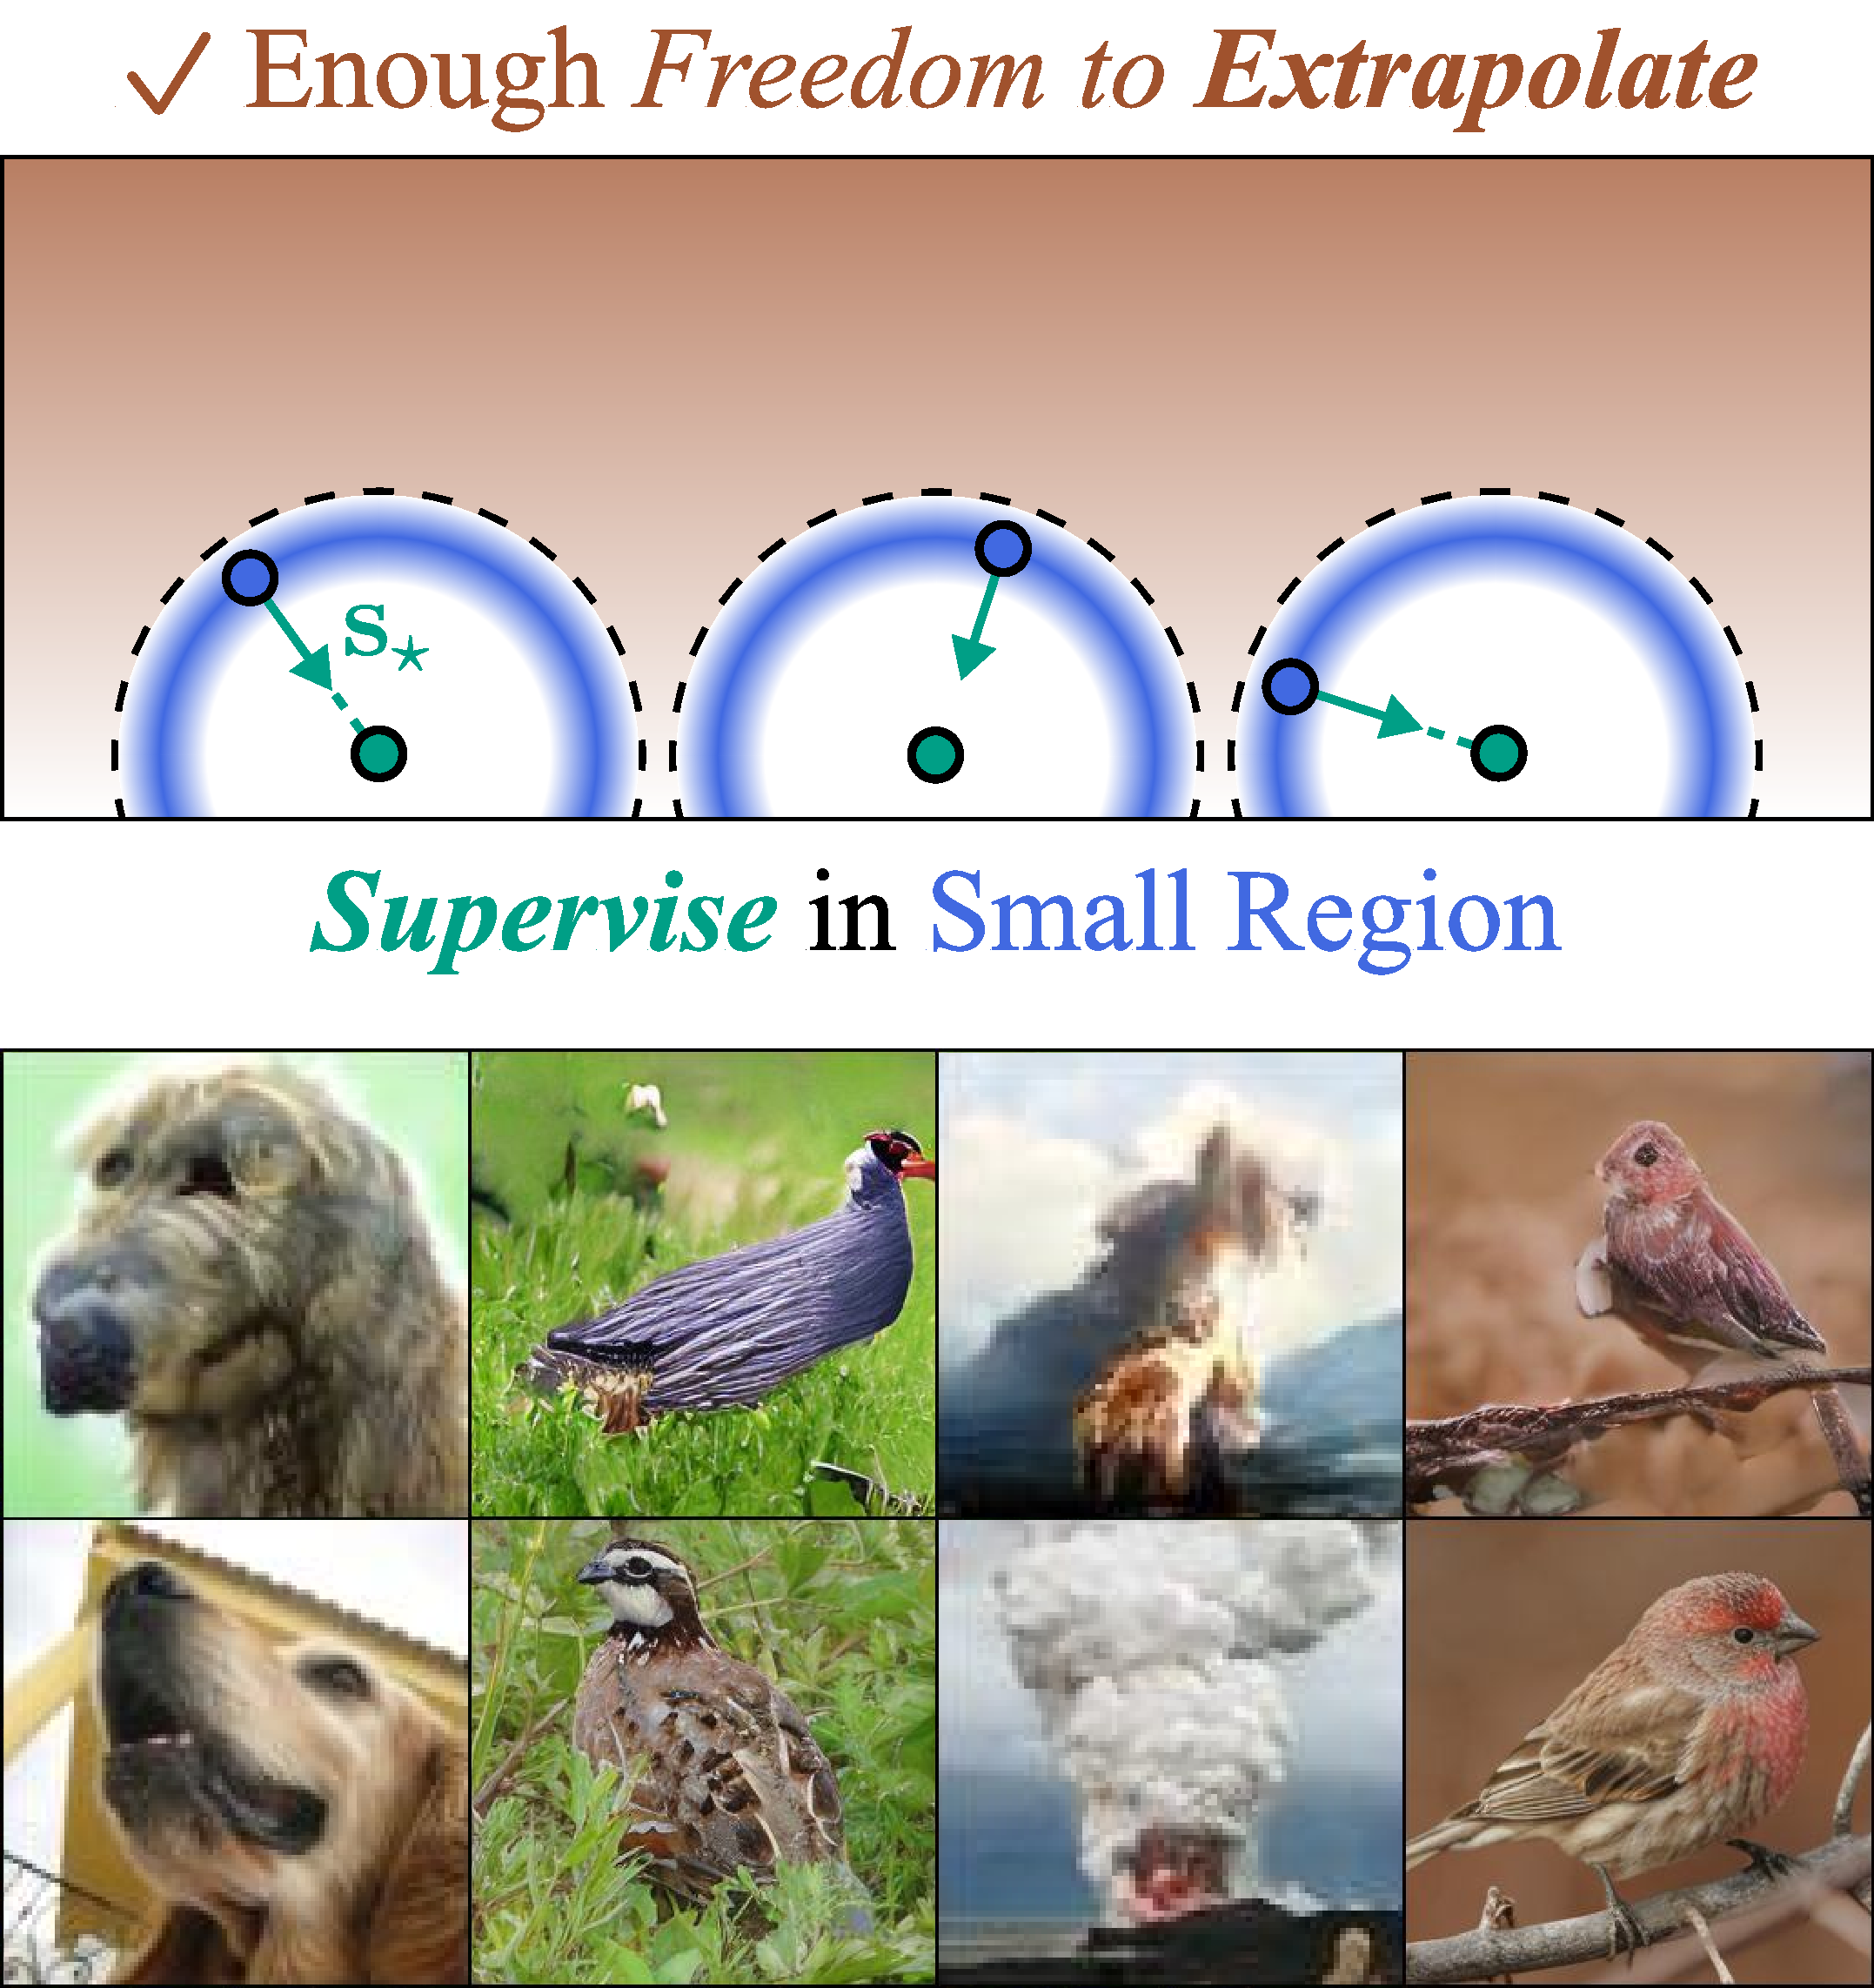
\includegraphics[height=0.99\textwidth]{figures/generalization/foe_generalization}
        \caption{\textbf{\xxpurple{Generalization.}} \xblue{Small supervision region} ($\trainrabsp = \trainsabsp$) \xsienna{ensures \emph{freedom to extrapolate}}.}
        \label{fig:foe-generalization}
    \end{subfigure}
    \hfill
    \begin{subfigure}[t]{0.32\textwidth}
        \centering
        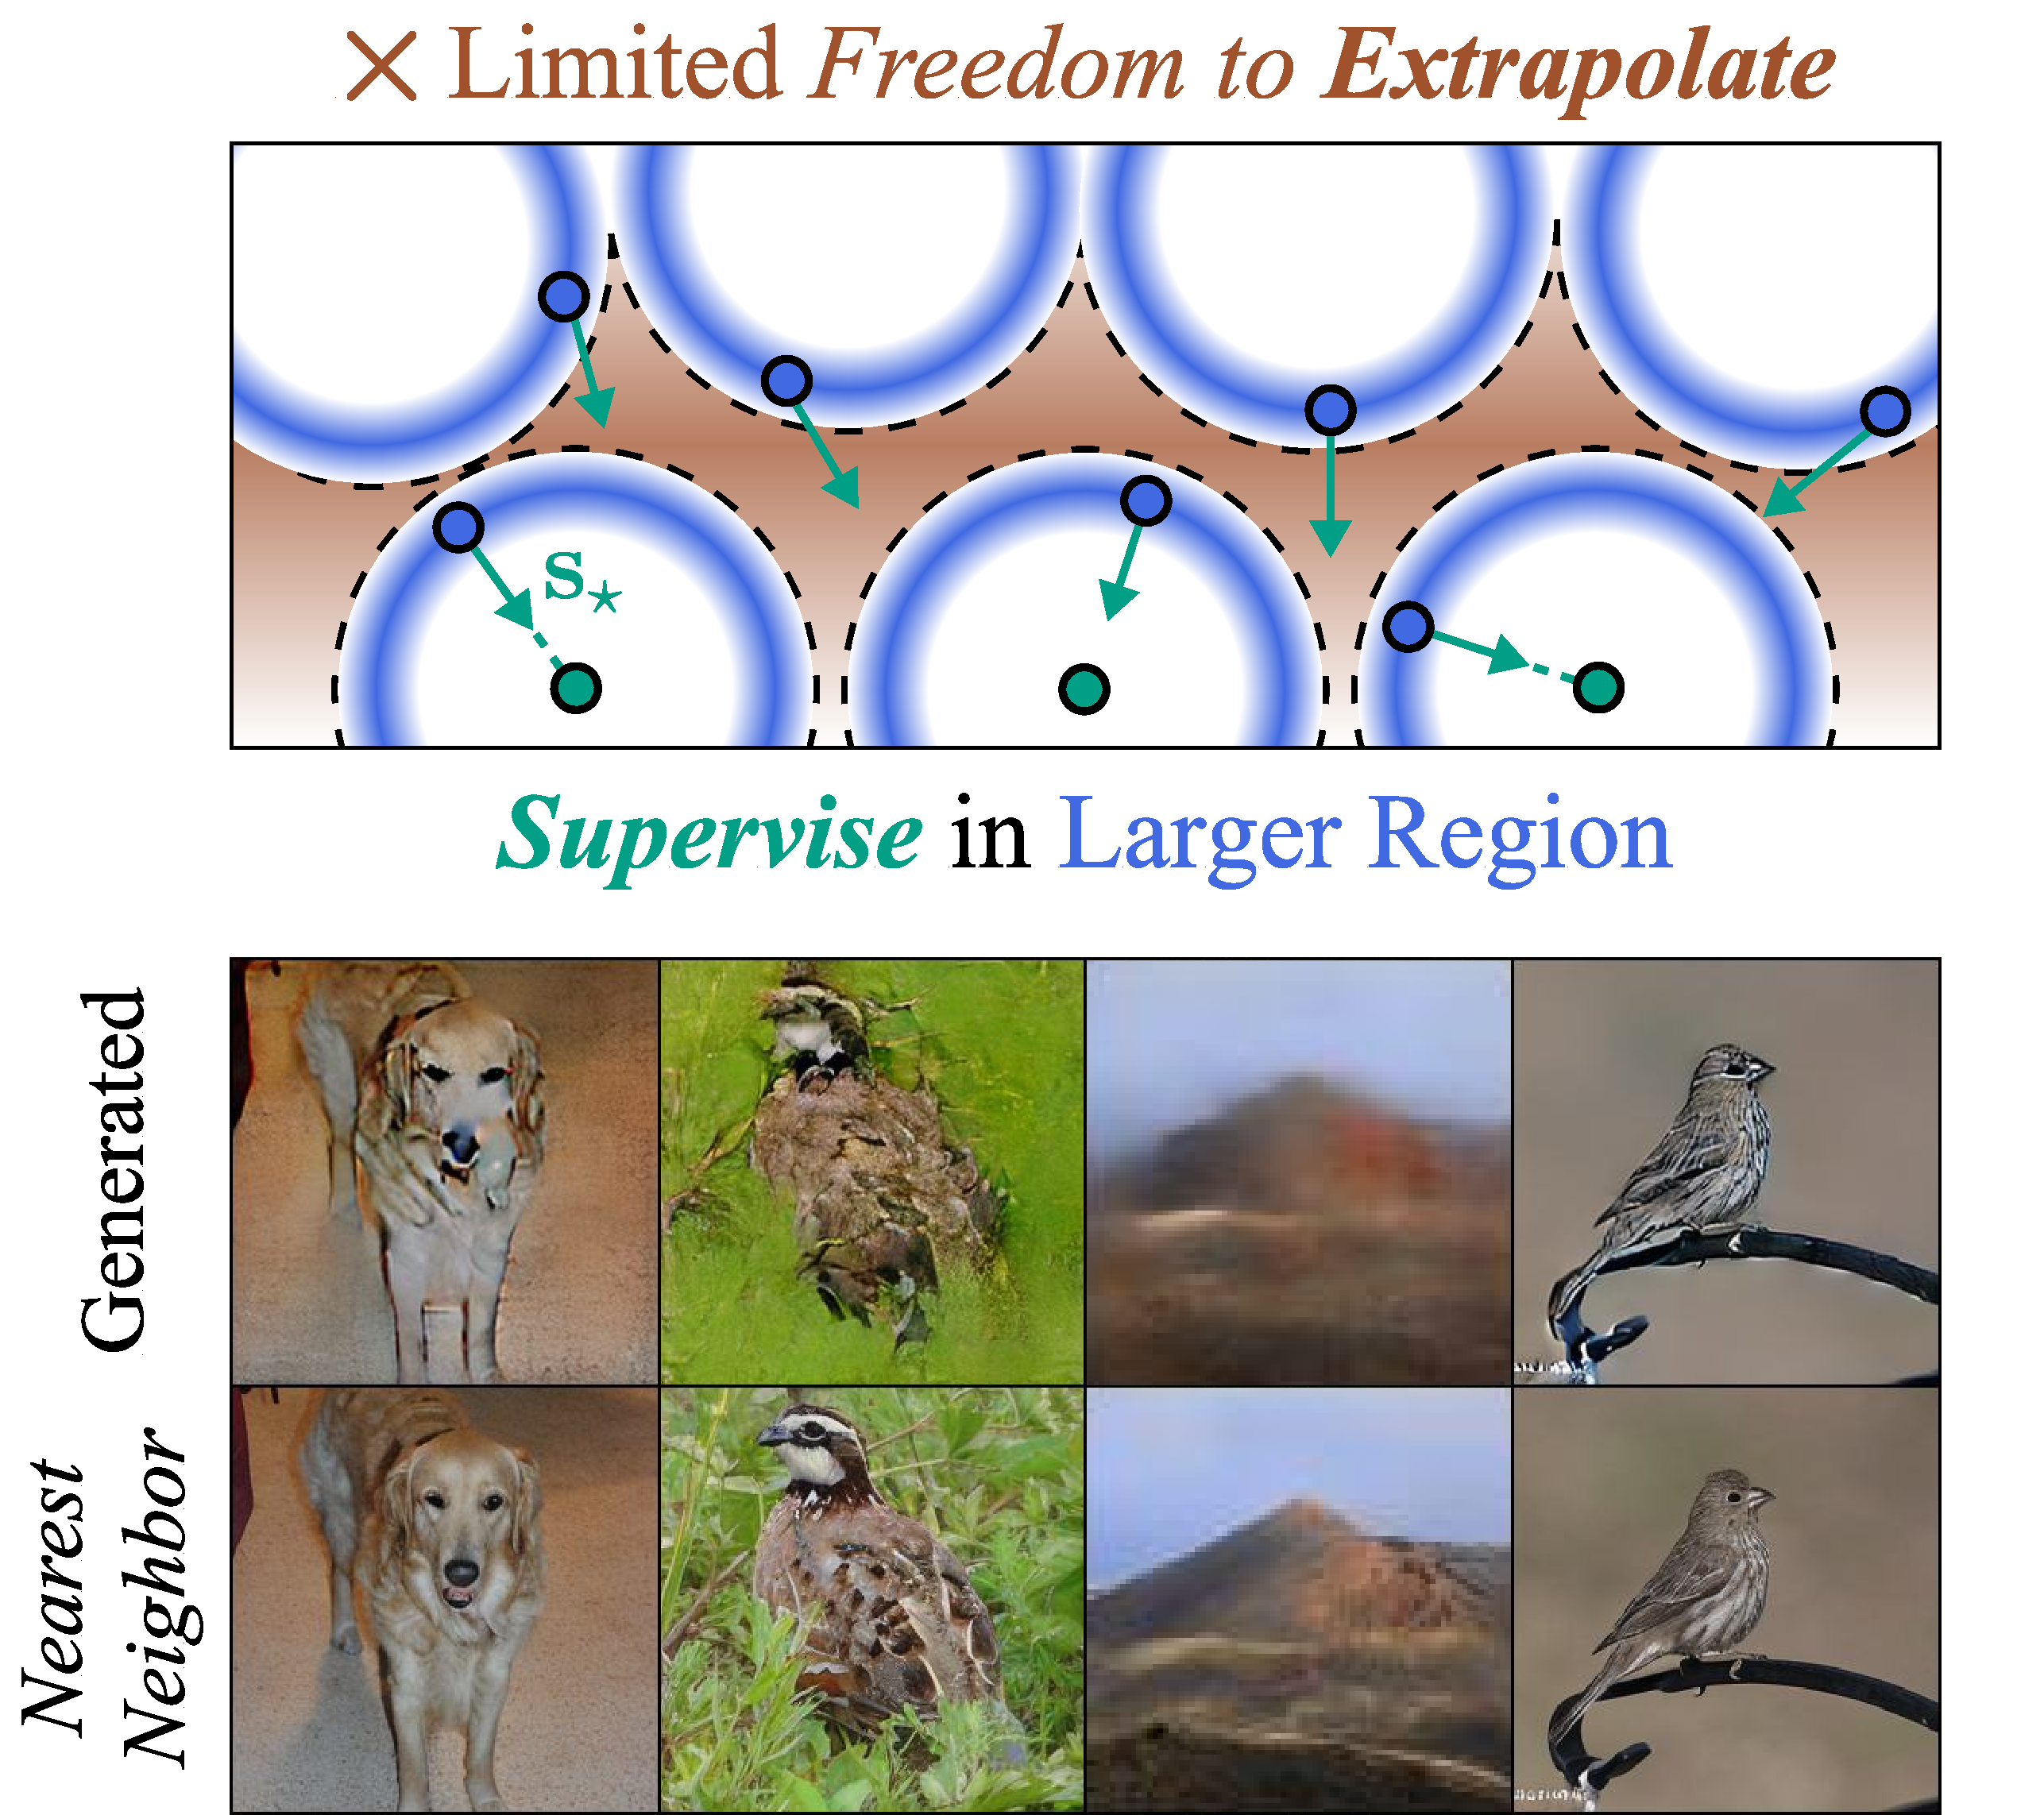
\includegraphics[height=0.99\textwidth,trim=4.1cm 0 0 0]{figures/generalization/foe_memorization}
        \caption{\textbf{\xolive{Memorization.}} \xblue{Larger supervision region} ($\trainrabsp \gg \trainsabsp$) \xsienna{limits \emph{freedom to extrapolate}}.}
        \label{fig:foe-memorization}
    \end{subfigure}
    \hfill
    \begin{subfigure}[t]{0.33\textwidth}
        \centering
        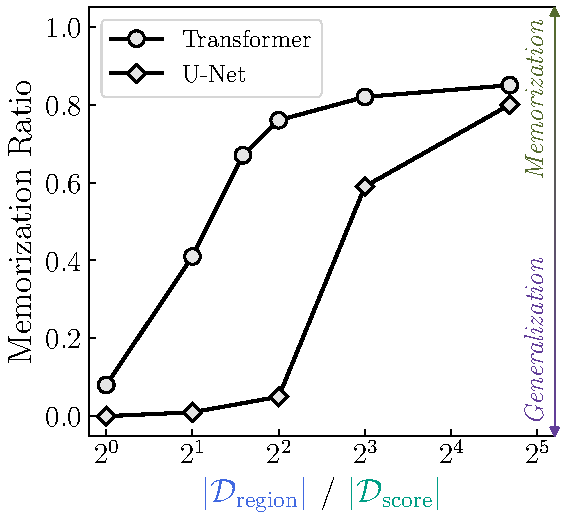
\includegraphics[height=0.85\textwidth,trim=0.2cm 0.15cm 0.3cm 0.45cm]{figures/generalization/foe_plot}
        \caption{\textbf{Quantitatively,} enlarging the supervision region $\trainr$ increases the ratio of \xolive{\emph{memorized}} samples.}
        \label{fig:foe-plot}
    \end{subfigure}
    \vskip -0.4\baselineskip
    \caption{\textbf{Experimental verification of \xsienna{\emph{freedom of extrapolation}} on ImageNet.} Deliberately limiting the \emph{freedom to extrapolate} transforms the diffusion model from \xxpurple{\emph{generalization}} to \xolive{\emph{memorization}}.}
    \label{fig:foe}
\end{figure}